\documentclass{article}
\usepackage[T1]{fontenc}
\usepackage[utf8]{inputenc}
\usepackage[a4paper, total={6in, 8in}]{geometry}
%\usepackage[icelandic]{babel}
\usepackage{graphicx} %package to manage images

\usepackage{hyperref}
\usepackage{siunitx}
\usepackage{tabularx}

\usepackage{xcolor}
\usepackage{listings}

\colorlet{mygray}{black!30}
\colorlet{mygreen}{green!60!blue}
\colorlet{mymauve}{red!60!blue}

\lstset{
  backgroundcolor=\color{gray!10},  
  basicstyle=\ttfamily,
  columns=fullflexible,
  breakatwhitespace=false,      
  breaklines=true,                
  captionpos=b,                    
  commentstyle=\color{mygreen}, 
  extendedchars=true,              
  frame=single,                   
  keepspaces=true,             
  keywordstyle=\color{blue},      
  language=c++,                 
  numbers=none,                
  numbersep=5pt,                   
  numberstyle=\tiny\color{blue}, 
  rulecolor=\color{mygray},        
  showspaces=false,               
  showtabs=false,                 
  stepnumber=5,                  
  stringstyle=\color{mymauve},    
  tabsize=3,                                     
  title=\lstname 
}

\title{Embedded Group Project\\ \large Project 2 - Speed Controller}

\author{Steinarr Hrafn Höskuldsson\\
Arnþór Gíslason\\
Andrew Madden\\
\\
Reykjavik University}
\date{September 2022}


\newcommand{\mycomment}[1]{}
\newcommand{\timerinterval}{5ms }

\begin{document}
\maketitle
 % how to comment, input image and code
\mycomment{
\begin{figure}[h]
    \centering
    \includegraphics[width=0.75\textwidth]{LAB3/Basic1.png}
    \caption{"Switch test" Breadboard set up}
    \label{fig:Switch_test}
\end{figure}

\lstinputlisting[caption=Defining 'ColorMatch' state, label={lst:colormatch}, language=Python, firstline=44, lastline=52]{LAB3/Basic.py}

}

\section{Part 1}
A timer was configured to run every \timerinterval and move the counted pulses into a separate variable called 'delta\_counts'. When the timer compares to the compare register a flag describing that the interrupt associated with the timer has run. 
When the main loops get a chance, it will take delta\_counts and calculate the rpm using function: 
\begin{equation}
     rpm = delta\_counts \cdot 60 / PPR \cdot INV\_DELTA\_T
\end{equation}

Where delta\_counts is the pulses counted during the \timerinterval period. PPR is how many pulses per revolution we expect, 28 in this case and INV\_DELTA\_T is inverse of \timerinterval, to get by without using floats or doubles in the program.

\section{Part 2}
\subsection{Measuring the time constant of the system}
The motor controller was wired according to the datasheet. The motor controller was fed motor power from an external power supply set to 6.0 V.
A program was written that sets the power going to the motor to full and then prints the rpm value of the output shaft every 10 ms.
The printed values can be seen in appendix \ref{appendix:motorspeedtable}. Python's matplotlib library was used to plot the values. From the plot we read that the motor reaches max speed of 65 RPM after around 170 ms and it reaches 63\% of max speed, 41 RPM, after 70 ms. Thus:
\[\tau = 70 \SI{}{\milli\second}\]
\begin{figure}[h]
    \centering
    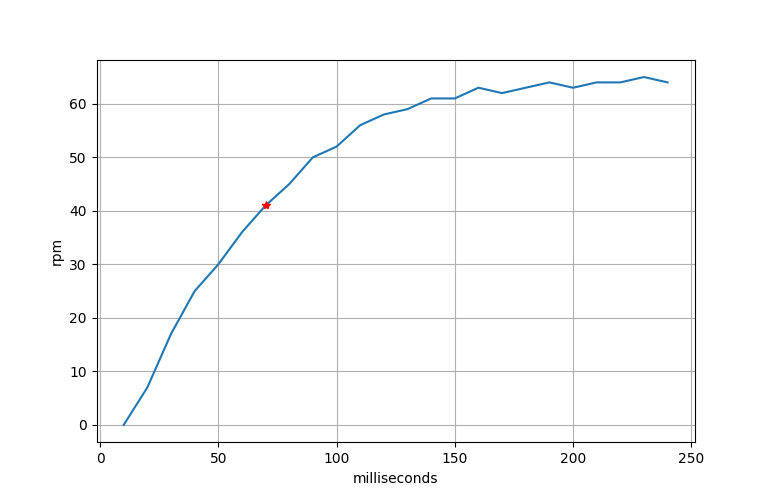
\includegraphics[width=0.75\textwidth]{Project2SpeedController/motor_response.png}
    \caption{Motor RPM plotted against time since power on}
    \label{fig:motor response}
\end{figure}
\subsection{Pulse width modulation}
The pulse width modulation was implemented using atmega328's Timer2 in phase correct PWM mode set at about 1kHz. The timer is 8bit which gives a resolution of about  0-255, where 0 is 0\% PWM and 255 is 100\% PWM. 

\maketitle

\begin{lstlisting}[caption=The relevant lines from the code used when measuring the motor response]
ISR(TIMER1_COMPA_vect)
{
  // happend every 10 ms.
  delta_counts = counter;
  counter = 0;
  flag = true;
}

void main(){
  flag = false;
  while (!flag){} // wait for flag
  // at this stage the counter just reset 
  pwm.set(255);// turn motor full on
  
  int i = 0; // to count ho many prints
  while (true)
  {
    // wait for flag
    if (flag){
      i++;
      flag = false;// set flag to false
      print_i(delta_counts); // print the speed
      // check if printing took too long
      if (flag){
        // if this happens then printing took longer than 10 ms and so the timer
        // reset, and we thus missed out on a rpm measurement, in that case
        // print '1' so it will be noticable
        print_i(1);
      }
    }
    if (i > 100) // print 100 times and then stop
      break;
  }
 
  while (true){} // do nothing forever
 }
\end{lstlisting}

\section*{Part 3}
The speed controller will have to update the speed to the motor at around $\frac{\tau}{10} = 7 ms$ giving an update frequency of around $143 Hz$

The speed controller will also have to :

\begin{itemize}
    \item Count encoder pulses
    \begin{description}
    The encoder pulses will be counted with interrupt sequences 
    \end{description}
    \item Compute speed using a stable time base
    \begin{description}
    To count the speed we will use a timer that fires an interrupt every 5ms at which point the encoder counter will be read and the speed calculated based on the change since last run.
    \end{description}
    \item Update the control output at a required rate
    \begin{description}
    The control output will be updated using the main loop, a flag will be set during the timer interrupt routine that will trigger the main loop to update the control output.
    \end{description}
    \item Stable PWM output at a suitable rate, observing
    \begin{description}
    The PWM output will be at a frequency of 1kHz. Thus fulfilling 
    \[ \frac{1}{f_{pwm}} \ll  \frac{1}{f_{update}} < \frac{\tau}{10}\]
    \[ \frac{1}{1000Hz} \ll \frac{1}{200Hz} < 7ms \]
    \end{description}

\end{itemize}

\section{Part 4}
A P\_controller class was implemented and a program that uses the controller class to control the speed of the motor was written. The code can be seen in Appendix [REF??]. 
The program keeps the set speed at 10.000 pulses per second for a few seconds and then drops it to 5.000 pulses per second. Meanwhile it prints the reference value, the measured value and the pwm output. A plot of the step response can be seen in Figure \ref{fig:step_response}.

\begin{figure}[h]
    \centering
    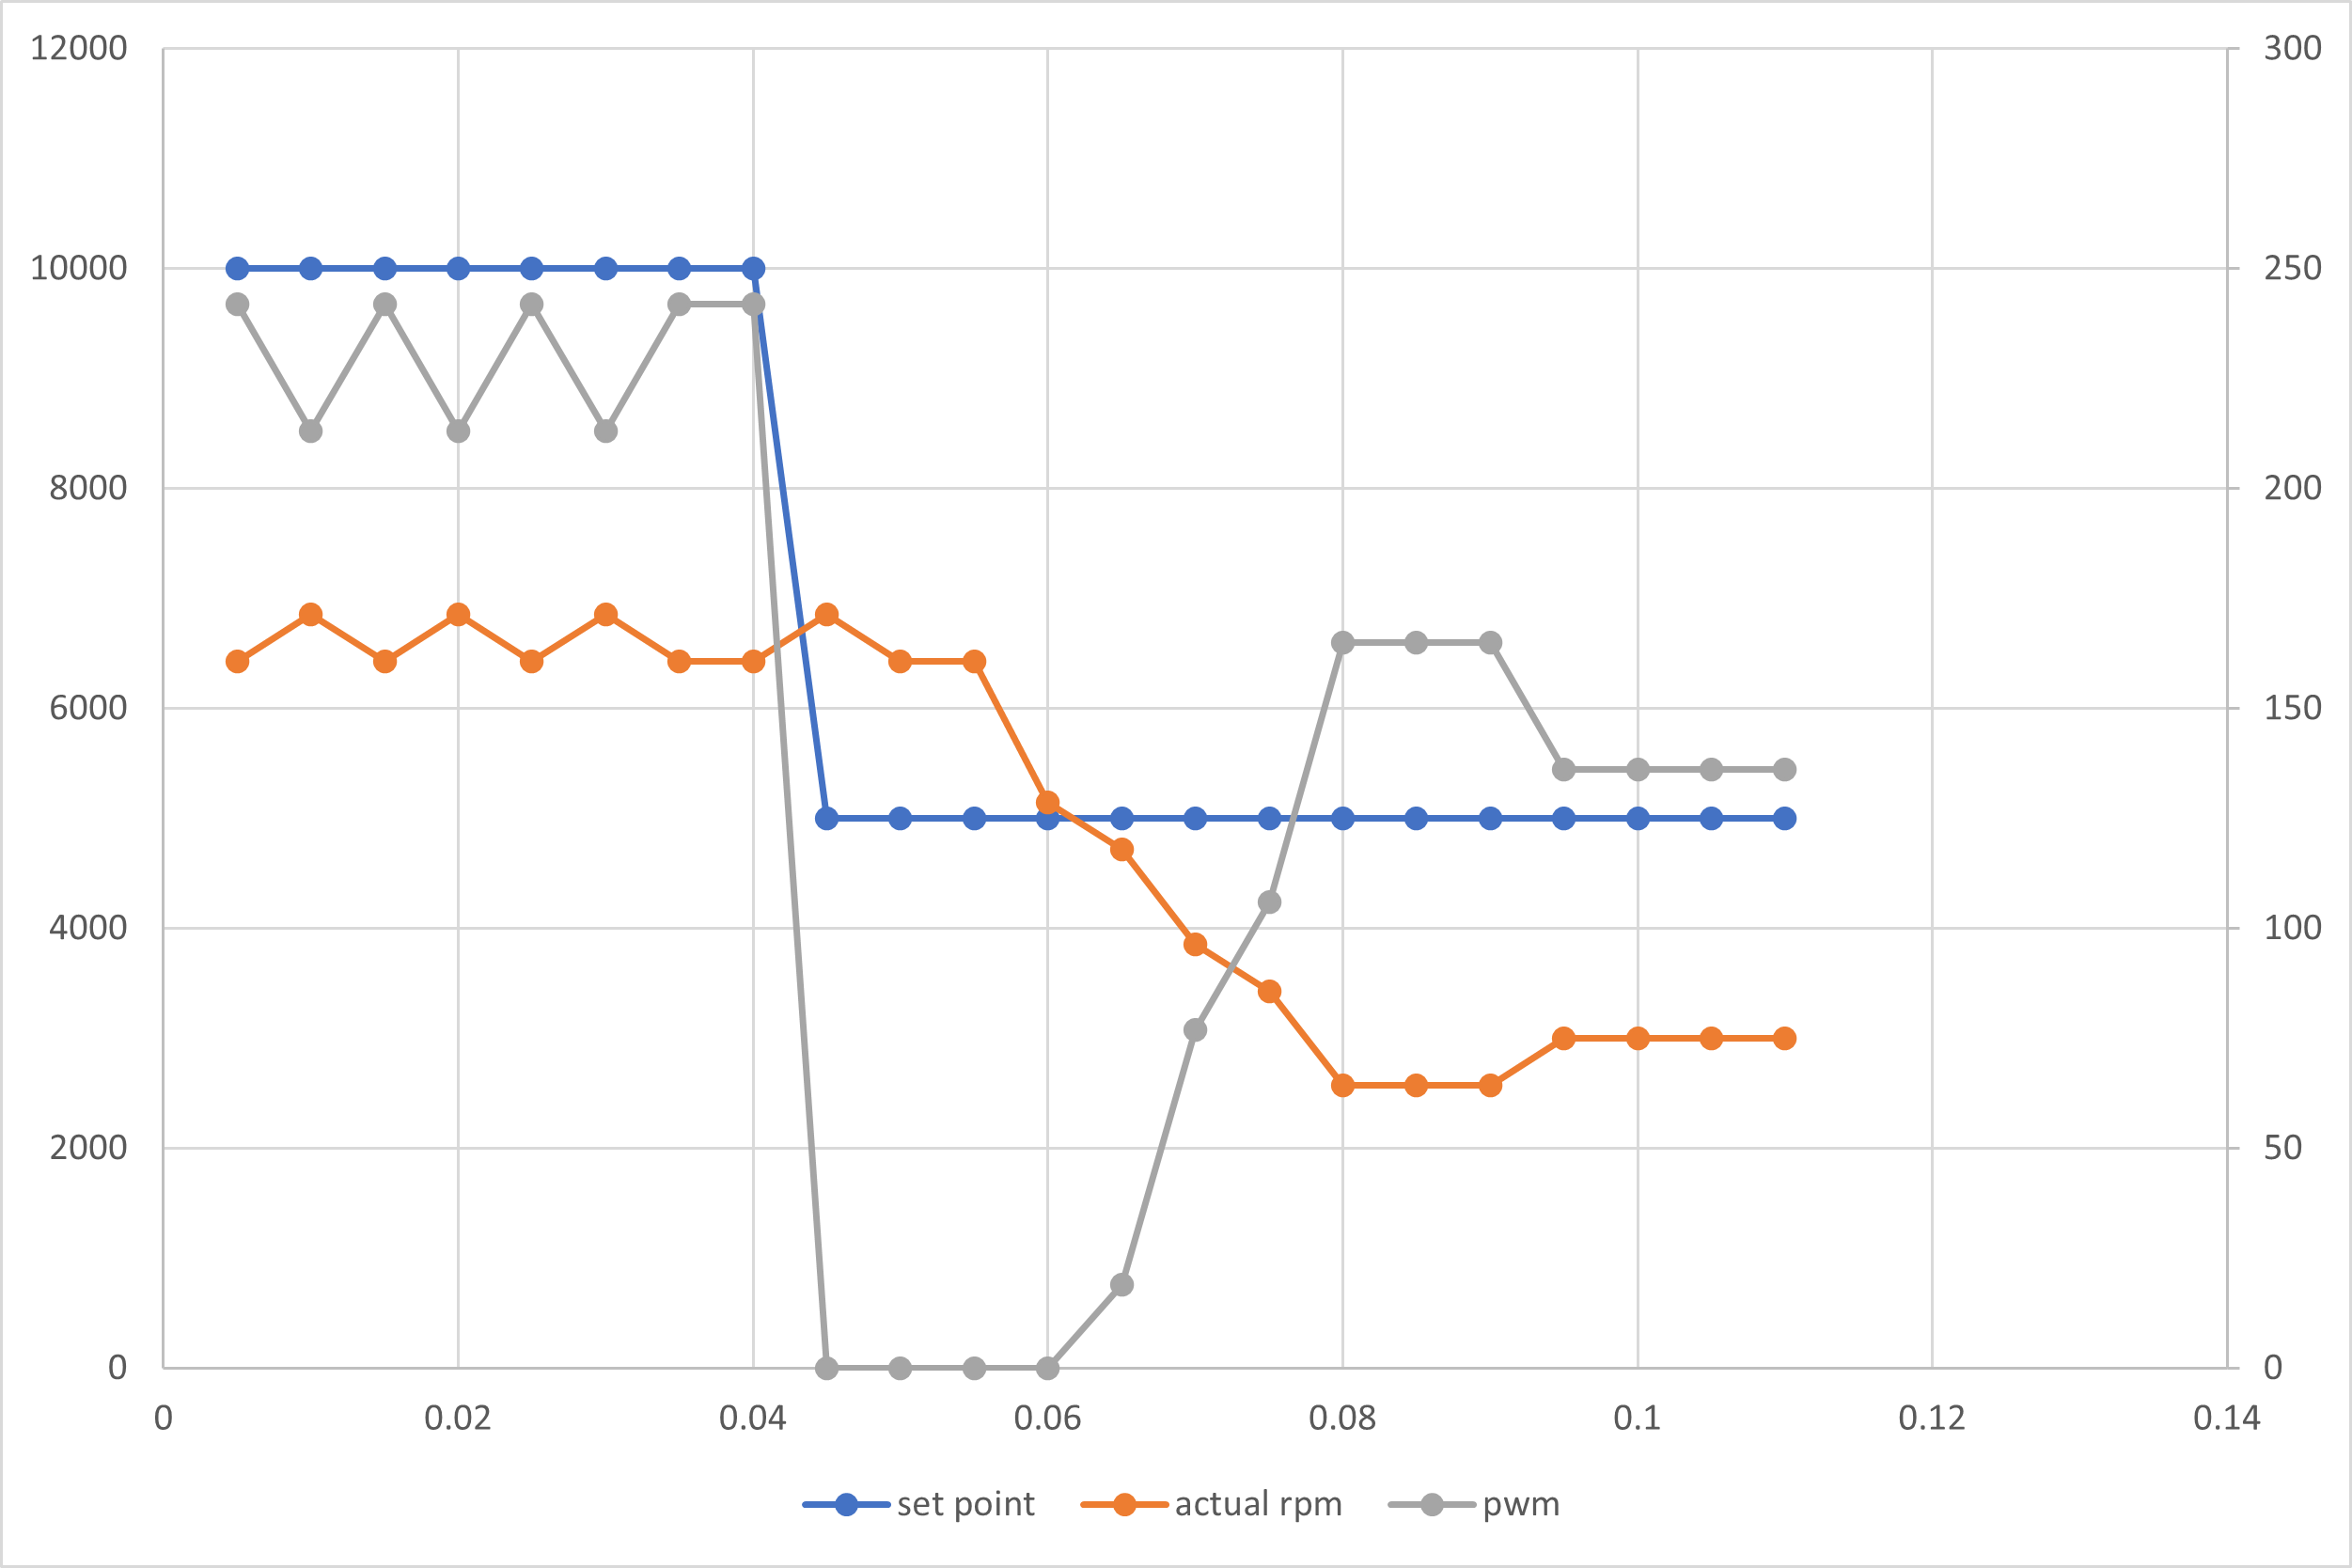
\includegraphics[width=0.75\textwidth]{Project2SpeedController/step_response2.png}
    \caption{Graph showing the step response of the motor when going from a higher to a lower set point. Set point and actual shown on the primary axis with pwm on the secondary axis}
    \label{fig:step_response}
\end{figure}

\section*{Appendix}
\appendix
\section{Motor Speed Up Measurements}\label{appendix:motorspeedtable}
\begin{table}[h]
\begin{tabular}{ll}
RPM & ms \\
0           & 10        \\
7           & 20        \\
17          & 30        \\
25          & 40        \\
30          & 50        \\
36          & 60        \\
41          & 70        \\
45          & 80        \\
50          & 90        \\
52          & 100       \\
56          & 110       \\
58          & 120       \\
59          & 130       \\
61          & 140       \\
61          & 150       \\
63          & 160       \\
62          & 170       \\
63          & 180       \\
64          & 190       \\
63          & 200       \\
64          & 210       \\
64          & 220       \\
65          & 230       \\
64          & 240      
\end{tabular}
\end{table}
\section{Code}\label{appendix:code}

This is not the correct code!

\lstinputlisting[caption=encoder\_simple.h]{Project1RotaryEncoder/src/encoder_simple.h}

\lstinputlisting[caption=timer\_msec.cpp]{Project1RotaryEncoder/src/encoder_simple.cpp}

\lstinputlisting[caption=main.cpp]{Project1RotaryEncoder/src/main.cpp}

\end{document}
